\chapter{مقدمه}

\section{ خونریزی درون‌جمجمه‌ای و اهمیت آن}

خونریزی‌ درون‌جمجمه‌ای
\LTRfootnote{Intracranial Hemorrhage}
یک وضعیت اضطراری پزشکی است که تشخیص سریع و دقیق آن به‌منظور درمان مؤثر بیمار و کاهش خطر ناتوانی شدید یا مرگ، حیاتی است \cite{grewal2018radnet}.
خونریزی درون جمجمه ای
می‌تواند به دلایل مختلفی از جمله آسیب مغزی تروماتیک
\LTRfootnote{Traumatic Brain Injury}
، بیماری‌های عروقی، یا مشکلات مادرزادی ایجاد شود و بر اساس محل خونریزی در مغز طبقه‌بندی می‌شود \cite{monica2022detection}.
 به‌صورت تقریبی سالانه بین 40000 تا 67000 بیمار دارای
خونریزی درون جمجمه ای
   در ایالات متحده آمریکا شناسایی می‌شوند که نرخ مرگ‌ومیر آنها در 30 روز اول حادثه در حدود 40 درصد است که در نتیجه آن، 
خونریزی درون جمجمه ای
   به یکی از بیماری‌ها با بیشترین آمار مرگ و میر تبدیل شده است. این در حالی است که عوارض دیگر این بیماری نیز بسیار خطرناک است، به‌عنوان‌مثال بیشتر از 46 درصد بیماران که دارای نوع خاصی از خونریزی درون‌جمجمه‌ای هستند، پس از بهبود به‌صورت دائمی دچار اختلالات شناختی می‌شوند
 \cite{arbabshirani2018advanced,burduja2020accurate,morgenstern2010guidelines,van2010incidence,hackett2000health}.

  باتوجه‌به نرخ بالای مرگ‌ومیر مرتبط با 
  خونریزی درون جمجمه ای
  ، تشخیص سریع و دقیق 
  خونریزی درون جمجمه ای
  با استفاده از روش‌های تصویربرداری ضروری است \cite{kuo2019expert}. سی‌تی‌اسکن
 \LTRfootnote{Computed Tomography Scan}
   شایع‌ترین روش برای تشخیص سریع خونریزی خصوصا در مراکز فوریت‌های پزشکی به‌حساب می‌آید که دقت مناسب را برای تشخیص این بیماری به متخصصین می‌دهد \cite{ye2019precise,grewal2018radnet,arbabshirani2018advanced,chilamkurthy2018deep}.


\section{انواع خونریزی درون‌جمجمه‌ای}
با پاره شدن عروق شریانی مغز، خون از درون عروق اصلی وارد بافت مغز می‌شود؛ این مسئله در حالی است که لخته‌شدن خون در داخل بدن سخت‌‌تر انجام می‌شود و به‌موجب آن خون وارد بافت مغز شده و با افزایش فشار داخل جمجمه، به بافت‌های حیاتی صدمات جدی وارد می‌کند.  
همان‌طور که در شکل
  \autoref{fig:ch1-brain-ich}
  مشخص است، با پاره شدن شریان‌های خونی درون مغز، خونی که وارد بافت مغز شده است و یک ضایعه بزرگ خونریزی را ایجاد کرده و این ضایعه در تصویر سی‌تی‌اسکن به‌صورت یک بافت که رنگ روشن‌تری نسبت به محیط اطراف دارد قابل‌شناسایی است.
   ‎
\begin{figure}[H]
\centering
\includegraphics[width=1.0\linewidth]{"Images/Chapter1/brain - ich"}
\caption{خونریزی درون‌جمجمه‌ای
\cite{healthjade_intracerebral_hemorrhage}}
\label{fig:ch1-brain-ich}
\end{figure}
خونریزی درون جمجمه‌ای متناسب با محل وقوع به زیرگروه‌های مختلفی تقسیم می‌شوند؛
این طبقه‌بندی شامل خونریزی اپیدورال
\lr{(EDH)}\LTRfootnote{Epidural}
 ، خونریزی ساب‌دورال
 \lr{(SDH)}\LTRfootnote{Subdural}
  ، خونریزی ساب‌آراکنوئید
 \lr{(SAH)}\LTRfootnote{Subarachnoid}
   ، خونریزی پارانشیم مغزی 
 \lr{(CPH)}\LTRfootnote{Cerebral Parenchymal}
   ، و خونریزی داخل بطنی
 \lr{(IVH)}\LTRfootnote{Intraventricular }
  است \cite{burduja2020accurate,hssayeni2020intracranial}.
  در
 \autoref{table: subtype}
 نمونه‌هایی از زیرگروه‌های خونریزی درون‌جمجمه‌ای، محل خونریزی، زمینه، علت وقوع، شکل و علائم بالینی نشان داده شده است؛ همانطور که از تصاویر مشخص است، تشخیص بعضی از انواع خونریزی ‌درون‌جممجه‌ای به علت حضور در اطراف بقیه بافت‌های مغز،‌ خصوصا جمجمه که از تراکم بیشتری برخوردار است و یا شکل پیچیده‌ای که دارند، حتی برای متخصصین نیز دشوار است.
  
  
\begin{table}[ht]
\centering
\adjustbox{max width=\textwidth,max totalheight=\textheight,keepaspectratio}{
\begin{tabular}{|c|p{7cm}|p{7cm}|p{7cm}|p{7cm}|p{7cm}|}
\hline
\textbf{} & \textbf{\lr{CPH}} & \textbf{\lr{IVH}} & \textbf{\lr{SAH}} & \textbf{\lr{SDH}} & \textbf{\lr{EDH}} \\ \hline
\textbf{محل} & داخل مغز & داخل بطن & بین عنکبوتیه و نرم‌شامه & بین سخت‌شامه و عنکبوتیه & بین سخت‌شامه و جمجمه \\ \hline
\textbf{تصویر} & 
\parbox[c][7cm][c]{7cm}{\centering 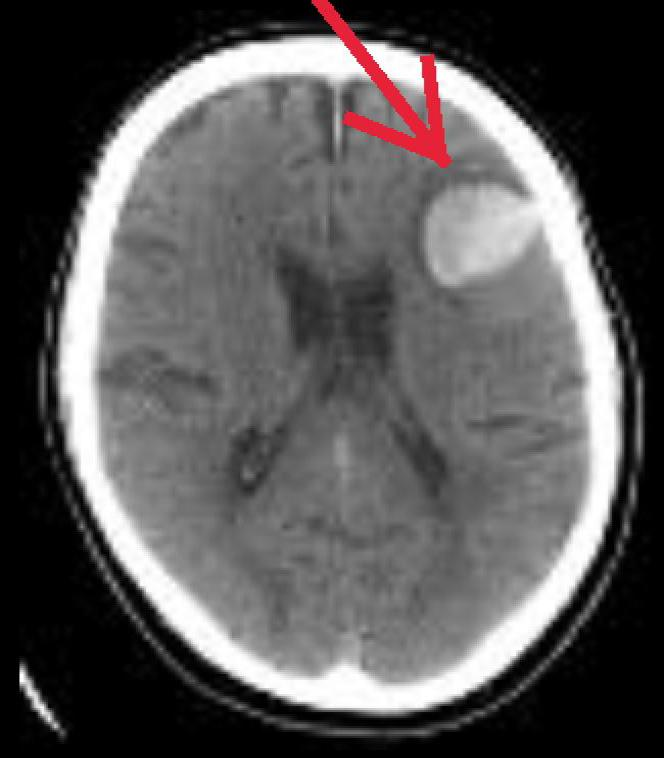
\includegraphics[width=6cm]{"Images/Chapter1/intraparenchymal.JPG"}} & 
\parbox[c][7cm][c]{7cm}{\centering 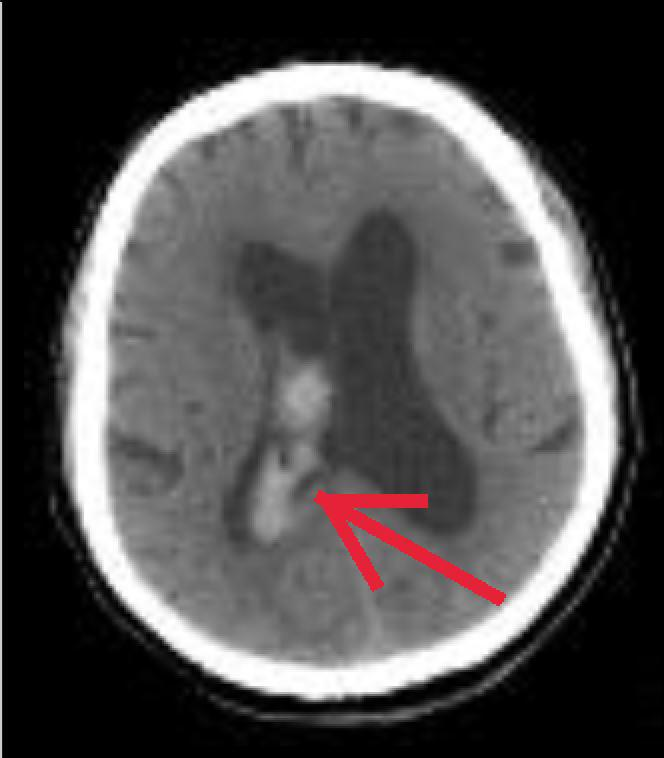
\includegraphics[width=6cm]{Images/Chapter1/intraventricular.JPG}} & 
\parbox[c][7cm][c]{7cm}{\centering 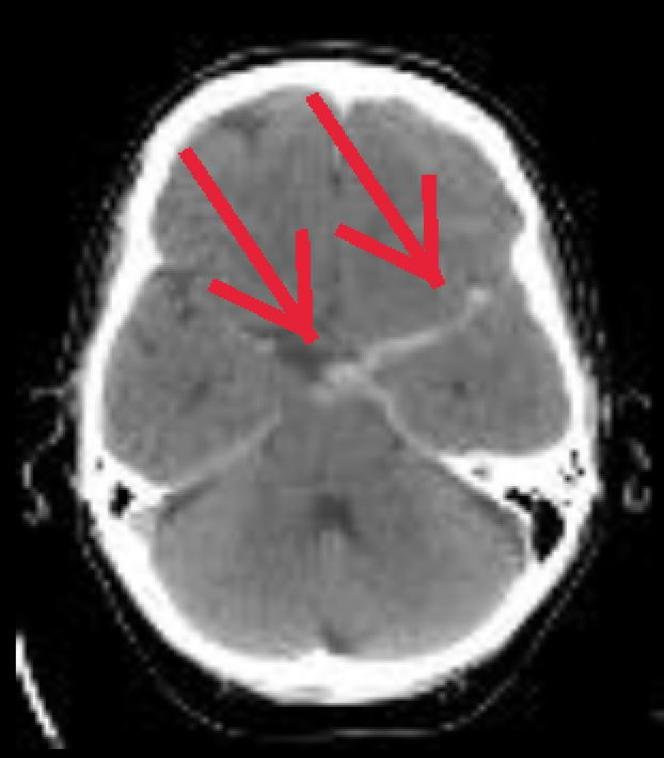
\includegraphics[width=6cm]{Images/Chapter1/subarachnoid.JPG}} & 
\parbox[c][7cm][c]{7cm}{\centering 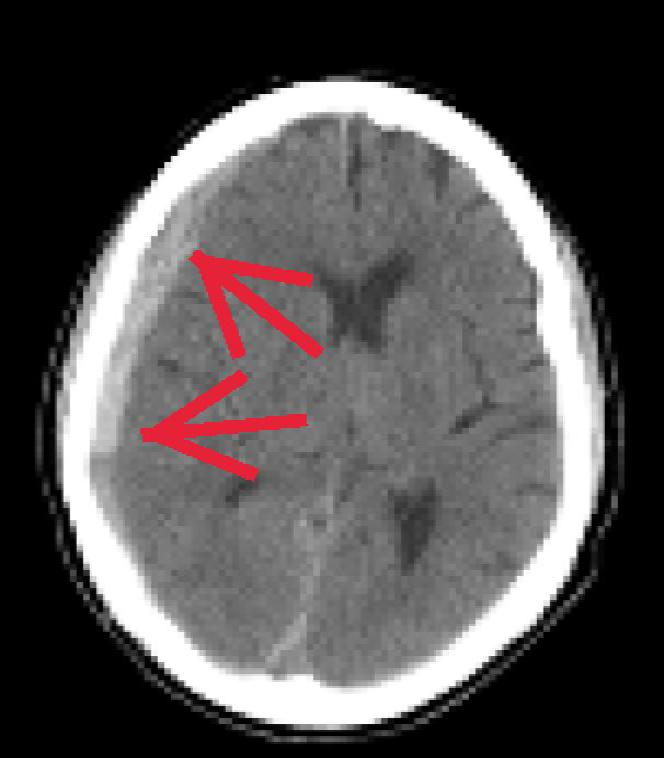
\includegraphics[width=6cm]{Images/Chapter1/subdural.JPG}} & 
\parbox[c][7cm][c]{7cm}{\centering 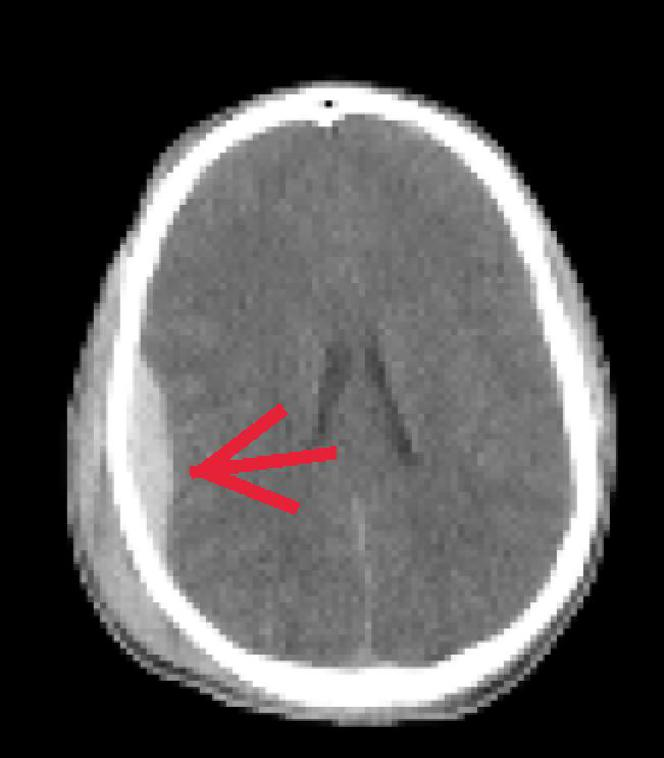
\includegraphics[width=6cm]{Images/Chapter1/Epidural.JPG}} \\ \hline
\textbf{زمینه‌ها} & فشار خون بالا، ضربه، ناهنجاری‌های شریانی-وریدی، تومور، و غیره & می‌تواند با خونریزی‌های درون‌مغزی و زیرعنکبوتیه همراه باشد & پارگی آنوریسم یا ناهنجاری‌های شریانی-وریدی یا ضربه & ضربه & ضربه یا پس از جراحی \\ \hline
\textbf{علت وقوع} & شریانی یا وریدی & شریانی یا وریدی & عمدتاً شریانی & وریدی (وریدهای پل‌زن) & شریانی \\ \hline
\textbf{شکل} & معمولاً گرد & مطابق با شکل بطن & در امتداد شیارها و شکاف‌ها & هلالی & عدسی‌شکل \\ \hline
\textbf{علائم بالینی} & حاد (شروع ناگهانی سردرد، حالت تهوع، استفراغ) & حاد (شروع ناگهانی سردرد، حالت تهوع، استفراغ) & حاد (بدترین سردرد زندگی) & ممکن است تدریجی باشد (بدتر شدن سردرد) & حاد (شکستگی جمجمه و تغییر وضعیت ذهنی) \\ \hline
\end{tabular}}
\caption{انواع زیرگروه‌های خونریزی درون‌جمجمه‌ای
\cite{rsna_hemorrhage_detection_kaggle}}
\label{table: subtype}
\end{table}

  
\section{روش‌های مرسوم در تشخیص خونریزی درون‌جمجمه‌ای}

در حال حاضر تصاویر سی‌تی‌اسکن، به‌عنوان استاندارد اصلی و غیرتهاجمی
\LTRfootnote{Non-invasive}
برای تشخیص خونریزی‌ درون‌جمجمه‌ای است. سی‌تی‌اسکن یک نوع تصویر پرتونگاری
\LTRfootnote{Radiography}
سه‌بعدی است که متشکل از تصاویر دوبعدی از اندام بدن است. روش عمومی پردازش تصاویر سی‌تی‌اسکن به‌صورت دستی انجام می‌پذیرد که به‌موجب آن متخصصین پرتونگاری
\LTRfootnote{Radiology}
 و پزشکی، با بررسی برش‌های
\LTRfootnote{ُSlice}
سی‌تی‌اسکن را به‌صورت مجزا بررسی می‌کنند و مناطق خونریزی را تشخیص می‌دهند. این فرایند به دلیل وابستگی به تخصص و تجربه فردی، شرایط محیطی و فشار کاری، زمان‌بر و مستعد خطا است. \cite{arbabshirani2018advanced,grewal2018radnet,ye2019precise,chilamkurthy2018deep,kuo2019expert}.
فرایند بررسی دستی تصاویر سی‌تی‌اسکن، زمان‌بر بوده و به‌شدت به دردسترس‌بودن پرتونگار‌های 
\LTRfootnote{Radiologist}
باتجربه بستگی دارد \cite{burduja2020accurate}.
 در شرایط اضطراری، خصوصا در مراکز فوریت‌های پزشکی، زمانی که برای پردازش برش‌های سی‌تی‌اسکن صرف می‌شود، می‌تواند به طور قابل‌توجهی در نتایج درمان بیمارها تأثیر بگذارد؛ این مسئله در مواردی از اهمیت بیشتری برخوردار می‌شود که درمان بیمار نیازمند مداخله فوری گروه پزشکی است \cite{chilamkurthy2018deep}. نکته حائز اهمیت در روش معمول برای بررسی تصاویر سی‌تی‌اسکن در مراکز پزشکی این است که بررسی اولیه تصاویر، توسط پزشکان و پرتونگار‌هایی با تجربه کمتر انجام می‌شود و در مراحل بعدی این تصاویر توسط متخصصینی با تجربه بیشتر بررسی می‌شود. تعدادی از مطالعات نشان داده‌اند که در روش مذکور،‌ بین پزشکان و پرتونگار‌هایی که در مرحله اول تصاویر را بررسی می‌کنند و پزشکان و پرتونگار‌هایی که در ادامه این تصاویر را بررسی می‌کنند،‌ اختلاف‌نظر وجود دارد که این مسئله می‌تواند منجر به عواقب جبران‌ناپذیر گردد
\cite{ye2019precise, alfaro1995accuracy, lal2000clinical, erly2002radiology, strub2007overnight}.
   احتمال خطای انسانی در بررسی دستی تصاویر پیچیده و سه‌بعدی سی‌تی‌اسکن، از دیگر نقاط ضعف روش معمول پردازش این تصاویر است، به‌ویژه در محیط‌های شلوغ و پرتنش که پرتونگار‌ها ممکن است تحت فشار زیاد باشند \cite{ye2019precise}.
   
\section{روش‌های رایانه‌ای در پردازش تصاویر پزشکی}
اهمیت مسئله خونریزی درون‌جمجمه‌ای و چالش‌های مرتبط با آن در بخش قبل مورد بررسی قرار گرفت، روش‌های مبتنی‌ بر پردازش رایانه‌ای
\LTRfootnote{Computer}
تصاویر پزشکی، می‌تواند یک راه‌حل مناسب برای رفع نقاط ضعف روش کنونی بررسی تصاویر پزشکی باشد
\cite{grewal2018radnet, arbabshirani2018advanced, ye2019precise, lee2019explainable, chang2018hybrid, chilamkurthy2018deep, titano2018automated, kuo2019expert}.
 ابزارهای خودکار برای تشخیص و کمیت‌سنجی خونریزی، از پیشرفت‌های روش‌های یادگیری ماشین 
\LTRfootnote{Machine Learning}
و یادگیری عمیق
\LTRfootnote{Deep Learning}
 و سامانه‌های
 \LTRfootnote{System}
  تشخیص به کمک رایانه 
 \LTRfootnote{Computer-aided Diagnosis}
 استفاده می‌کنند تا تجزیه‌وتحلیل سریع و دقیقی از تصاویر سی‌تی‌اسکن ارائه دهند. با خودکارسازی تشخیص خونریزی درون‌جمجمه‌ای و استفاده از آنها به‌صورت نظر ثانویه
  \LTRfootnote{ُSecond Opinion}
 ، این سامانه‌ها می‌توانند بار کاری پرتونگار‌ها را کاهش دهند، دقت تشخیص را افزایش دهند از اشتباهات متخصصین جلوگیری کنند، زمان تشخیص را به حداقل برسانند، بعضی از هزینه‌های فرایند درمان را به علت کاهش دخالت انسانی کاهش دهند و به‌صورت کلی فرایند تشخیص را بهبود ببخشند که این موارد به بهبود نتایج بیماران منجر خواهد شد. بااین‌حال، ضمن اینکه سامانه‌های تشخیص به کمک رایانه نویدبخش هستند؛ اما امکان خطا در آنها وجود دارد که می‌تواند تصمیم‌گیری بالینی را با مشکلاتی روبرو کند؛ بنابراین، ادغام این ابزارها در عمل باید با دقت انجام شود \cite{titano2018automated}.
